\section*{Appendix}
\appendix

\begin{comment}
Appendix: Put all Figures, Tables, Algorithms, etc., in appendix.

\section{First Appendix}
\label{app:FirstAppendix}

\begin{figure}[tbh]

\includegraphics[width=.45\textwidth]{Images/sdu-logo.png}
\caption{SDU Logo}
\label{app:fig:SDULogo}
\end{figure}

\section{Second Appendix}
\label{app:SecondAppendix}

\begin{figure*}[tbh]

\includegraphics[width=.95\textwidth]{Images/sdu-logo.png}
\caption{Full width figure SDU Logo}
\label{app:fig:SDULogoV2}
\end{figure*}
\end{comment}

\section{Source Code and Assets}
main version: https://github.com/Vimian/smart-door-lock
\newline
BLE version: https://github.com/Vimian/smart-door-lock/tree/master-ble

\section{Wiring Diagram}
\label{app:WiringDiagram}

\begin{figure*}[tbh]
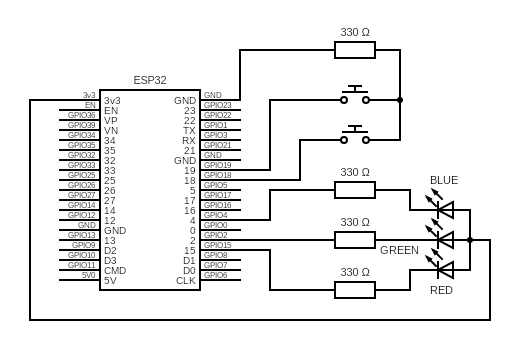
\includegraphics[width=.95\textwidth]{./../circuit/circuit.png}
\caption{Hardware wiring diagram}
\label{app:fig:WiringDiagram}
\end{figure*}

\section{UPPAAL Models}
\label{app:UPPAALModels}

\begin{figure*}[tbh]
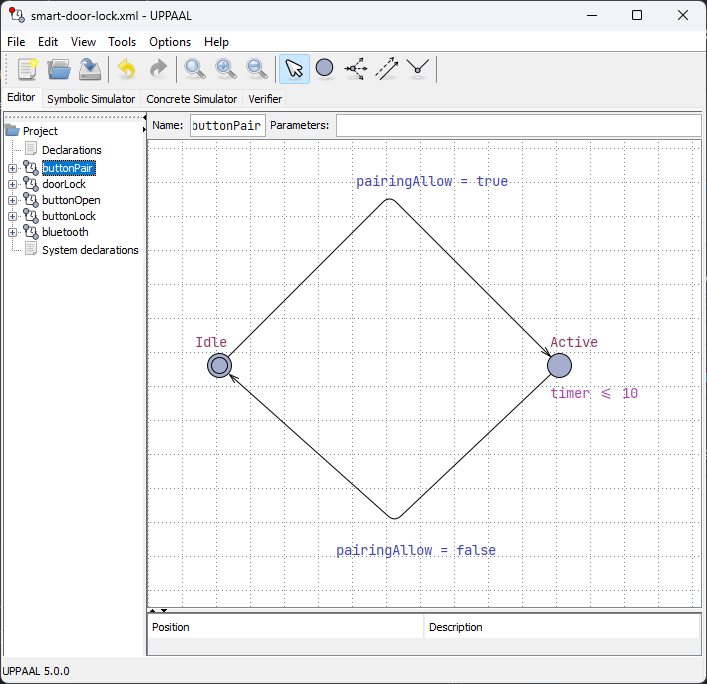
\includegraphics[width=.45\textwidth]{./../uppaal/buttonPair.png}
\caption{UPPAAL model of the pairing button}
\label{app:fig:UPPAALModelButtonPair}
\end{figure*}

\begin{figure*}[tbh]
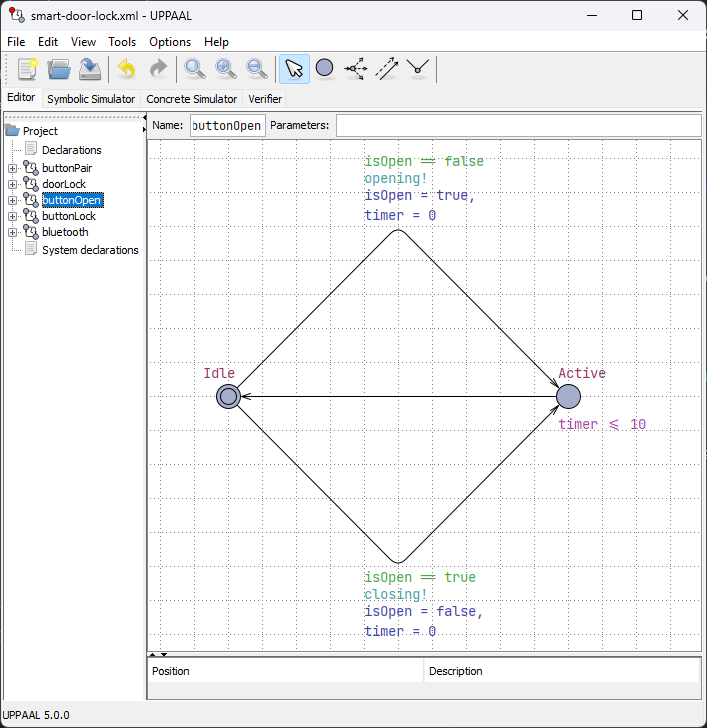
\includegraphics[width=.45\textwidth]{./../uppaal/buttonOpen.png}
\caption{UPPAAL model of the open and close button}
\label{app:fig:UPPAALModelButtonOpen}
\end{figure*}

\begin{figure*}[tbh]
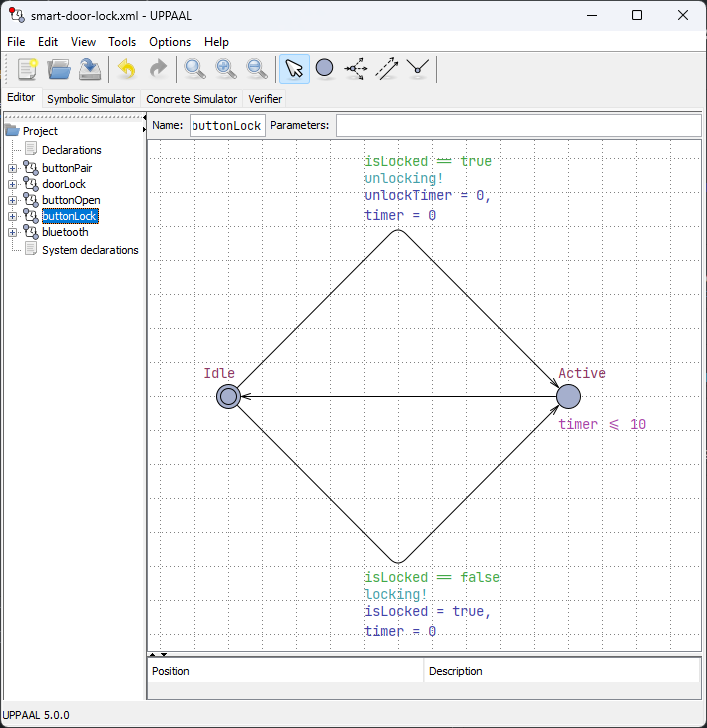
\includegraphics[width=.45\textwidth]{./../uppaal/buttonLock.png}
\caption{UPPAAL model of the lock and unlock button}
\label{app:fig:UPPAALModelButtonLock}
\end{figure*}

\begin{figure*}[tbh]
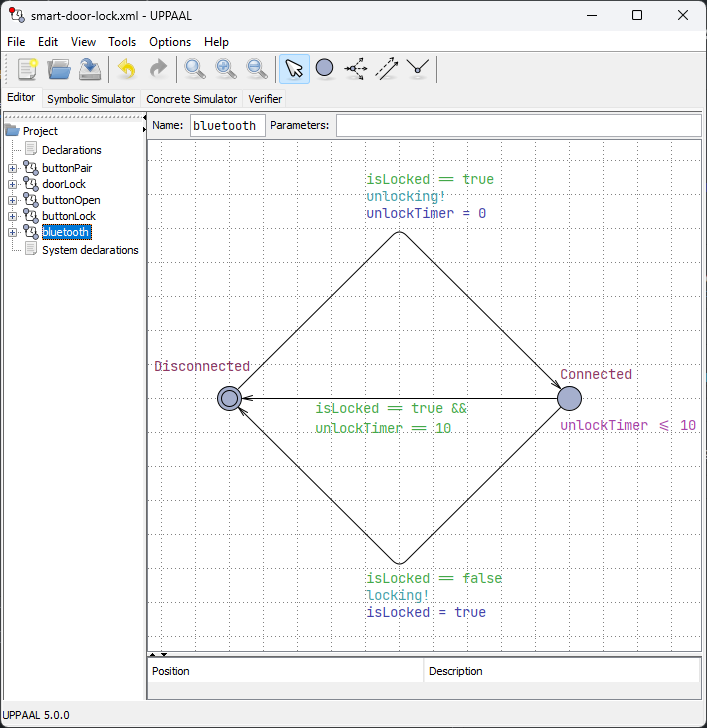
\includegraphics[width=.45\textwidth]{./../uppaal/bluetooth.png}
\caption{UPPAAL model of bluetooth}
\label{app:fig:UPPAALModelBluetooth}
\end{figure*}

\begin{figure*}[tbh]
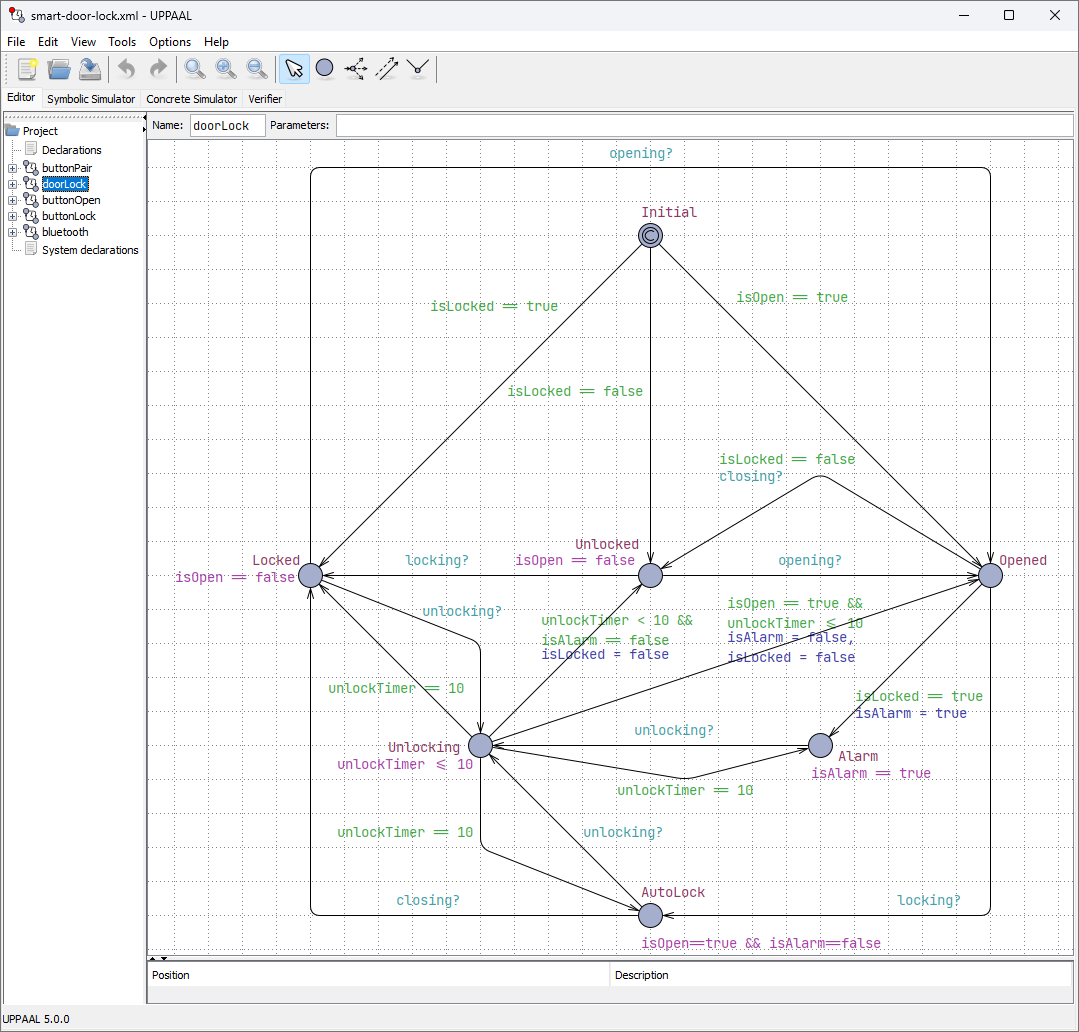
\includegraphics[width=.95\textwidth]{./../uppaal/doorLock.png}
\caption{UPPAAL model of the door lock}
\label{app:fig:UPPAALModelDoorLock}
\end{figure*}

\section{Validation Tests}
\label{app:ValidationTests}

\begin{figure*}[tbh]
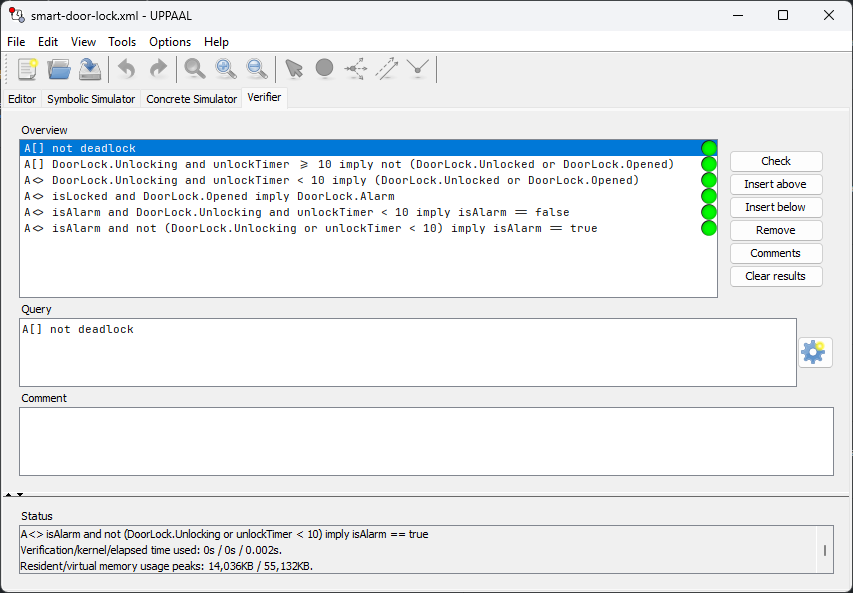
\includegraphics[width=.95\textwidth]{./../uppaal/tests.png}
\caption{UPPAAL tests}
\label{app:fig:UPPAALTests}
\end{figure*}

\section{LED Colors}
\label{app:LEDColors}
None - unlocked and closed
\newline
Green - locked and closed
\newline
red - unlocked and open
\newline
yellow - locked and open
\newline
yellow/white - locked, open and alarm
\newline
green/cyan - locked, closed and alarm
\newline
! purple - unlocked, open and alarm
\newline
! blue - alarm
\newline
! are states that does not exist in the UPPAAL models.